\documentclass[a4paper]{scrreprt}

% Uncomment to optimize for double-sided printing.
% \KOMAoptions{twoside}

% Set binding correction manually, if known.
% \KOMAoptions{BCOR=2cm}

% Localization options
\usepackage[english]{babel}
\usepackage[T1]{fontenc}
\usepackage[utf8]{inputenc}

% Sub figures
\usepackage{subcaption}

% Quotations
\usepackage{dirtytalk}

% Floats
\usepackage{float}

% Enhanced verbatim sections. We're mainly interested in
% \verbatiminput though.
\usepackage{verbatim}

% Automatically remove leading whitespace in lstlisting
\usepackage{lstautogobble}

% CSV to tables
\usepackage{csvsimple}

% PDF-compatible landscape mode.
% Makes PDF viewers show the page rotated by 90°.
\usepackage{pdflscape}

% Advanced tables
\usepackage{array}
\usepackage{tabularx}
\usepackage{longtable}

% Fancy tablerules
\usepackage{booktabs}

% Graphics
\usepackage{graphicx}

% Current time
\usepackage[useregional=numeric]{datetime2}

% Float barriers.
% Automatically add a FloatBarrier to each \section
\usepackage[section]{placeins}

% Custom header and footer
\usepackage{fancyhdr}

\usepackage{geometry}
\usepackage{layout}

% Math tools
\usepackage{mathtools}
% Math symbols
\usepackage{amsmath,amsfonts,amssymb}
\usepackage{amsthm}
% General symbols
\usepackage{stmaryrd}

% Utilities for quotations
\usepackage{csquotes}

% Bibliography
\usepackage[
  style=alphabetic,
  backend=biber, % Default backend, just listed for completness
  sorting=ynt % Sort by year, name, title
]{biblatex}
\addbibresource{references.bib}

\DeclarePairedDelimiter\abs{\lvert}{\rvert}
\DeclarePairedDelimiter\floor{\lfloor}{\rfloor}

% Bullet point
\newcommand{\tabitem}{~~\llap{\textbullet}~~}

\pagestyle{plain}
% \fancyhf{}
% \lhead{}
% \lfoot{}
% \rfoot{}
% 
% Source code & highlighting
\usepackage{listings}

% SI units
\usepackage[binary-units=true]{siunitx}
\DeclareSIUnit\cycles{cycles}

\newcommand{\lecture}{61062 - Computer Vision}
% Convenience commands
\newcommand{\mailsubject}{\lecture - Assignemt 02, Part 02}
\newcommand{\maillink}[1]{\href{mailto:#1?subject=\mailsubject}
                               {#1}}

% Should use this command wherever the print date is mentioned.
\newcommand{\printdate}{\today}

\subject{\lecture}
\title{Assignment 02, Part 02}

\author{Michael Senn \maillink{michael.senn@students.unibe.ch} --- 16-126-880}

\date{\printdate}

% Needs to be the last command in the preamble, for one reason or
% another. 
\usepackage{hyperref}

\begin{document}
\maketitle

\chapter{Introduction}

The goal of the assignment was to reconstruct a 3D model given a set of 2D
point correspondences. These 2D point correspondences were the result of two
images taken of an object from two different cameras.

As the point correspondences were noisy, outliers had to be eliminated by means
of the RANSAC algorithm. \autocite{fischlerRandomSampleConsensus1981}

\chapter{Methods}

\section{Elimination of outliers using RANSAC}

In a first step, outliers were eliminated by means of the RANSAC algorithm.
\autocite{fischlerRandomSampleConsensus1981} Summarizing, a random set of eight
points was selected and the fundamental matrix estimated by means of the
normalized eight-point algorithm
\autocite{hartleyDefenseEightpointAlgorithm1997}. This process was repeated a
fixed amount of times, and the fundamental matrix which lead to the lowest
sum-of-squared errors between predicted and actual positions was used further.

The fundamental matrix was then optimized by iteratively applying the
normalized eight-point algorithm until the determined inliers, until the set of
inliers did not change any further.

\section{Calculation of essential matrix from fundamental matrix}

Using the provided calibration matrix $K$ of the cameras, and the earlier
calculated fundamental matrix $F$, the essential matrix $E$ was calculated as:

\[
		E = K^T F K
\]

\section{Decomposition of essential matrix into rotation matrix and translation vector}

The rotation matrix $R$ and translation vector $t$ were then extracted from the
essential matrix $E$ as described by Hartley and Zisserman
\autocite{hartleyMultipleViewGeometry2003}. Summarizing, SVD was used to
decompose $U \Sigma V^T = E$. $U, V^T \in SO(3)$ was enforced by multiplying $U$
and $V^T$ with $-1$ respectively if their determinat was negative. Then, the two
possible rotation matrices $R_1$ and $R_2$, as well as the two possible
translaction vectors $t_1$ and $t_2$ followed:

\begin{align*}
		W & = \begin{pmatrix}
				0 & 1 & 0 \\
				-1 & 0 & 0 \\
				0 & 0 & 1
		\end{pmatrix} \\
		R_1 & = U W V^T \\
		R_2 & = U W^T V^T \\
		t_1 & = -u_3 \\
		t_2 & = u_3
\end{align*}

Where $u_3$ is the third column of $U$.

The provided code then calculated which of the four possible camera matrices is
the valid one.

\section{Evaluating accuracy of estimated rotation and translation}

Using the provided ground truth data containing the rotation matrices and
translation vectors of the two cameras, the actual rotation matrix and
translation vector of the transformation between the two cameras was
calculated. These were then compared with the estimated ones by means of the L1
norm, where the rotation matrices were first converted to Euler angles.

\chapter{Results}

Figure \ref{fig:cow} shows the reconstruction of the object --- in this case a
cow. Clearly the reconstruction looks quite decent by eye.

\begin{figure}
		\centering
		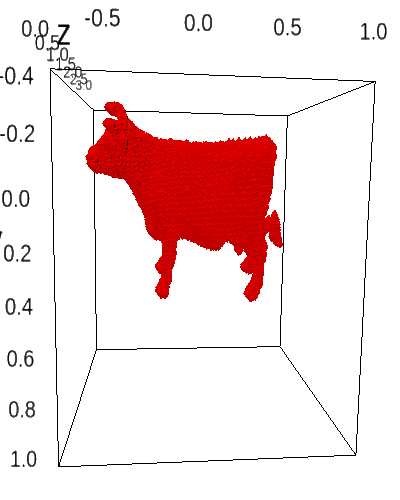
\includegraphics[width=0.5\textwidth]{resources/cow.png}
		\caption{Reconstruction of cow}
		\label{fig:cow}
\end{figure}

Table \ref{tbl:errors} then also lists the L1 norm of the differences between
the estimated and actual rotation matrix and translation vector. The errors
being rather low further confirms that the reconstruction process went over
fairly well.

\begin{table}
		\centering
		\begin{tabular}{ll}
				\toprule
				Component & L1 norm of error \\
				\midrule
				Rotation matrix & $\approx 0.0615$ \\
				Translation vector & $\approx 0.0074$ \\
				\bottomrule
		\end{tabular}
		\caption{L1 norm of error of estimated camera components}
		\label{tbl:errors}
\end{table}

\printbibliography

\end{document}
